\documentclass{article}
\usepackage{fullpage}
\usepackage{multicol,multirow}
\usepackage{tabularx}
\usepackage{ulem}
\usepackage[utf8]{inputenc}
\usepackage[russian]{babel}
\usepackage{pgfplots}
\usepackage{graphicx}

\begin{document}

\section*{Лабораторная работа №8 по курсу «Численные методы»}

Выполнил студент группы М8О-408Б-20 Попов Матвей.
\\
Преподаватель: Пивоваров Д.\,Е.

\subsection*{Цель}

Используя схемы переменных направлений и дробных шагов, решить двумерную 
начально-краевую задачу для дифференциального уравнения параболического типа. 
В различные моменты времени вычислить погрешность численного решения путем 
сравнения результатов с приведенным в задании аналитическим решением $U(x, t)$. 
Исследовать зависимость погрешности от сеточных параметров $\tau, h_x, h_y$.

\subsection*{Вариант 1}
% $$ \frac{\partial^2 u}{\partial x^2} + \frac{\partial^2 u}{\partial y^2} = 0 $$
% $$ u(0, y) = y $$
% $$ u(1, y) = 1 + y $$
% $$ u(x, 0) = x $$
% $$ u(x, 1) = 1 + x $$
% Аналитическое решение: $$ U(x, y) = x + y $$
$$\frac{\partial u}{\partial t} = a \frac{\partial^2 u}{\partial x^2} + a \frac{\partial^2 u}{\partial y^2}, a > 0$$
$$u(0,y,t) = \cos{(\mu_2y)}\exp{(-(\mu_1^2 + \mu_2^2)at)}$$
$$u(\pi,y,t) = (-1)^{\mu_1}\cos{(\mu_2 y)}\exp{(-(\mu_1^2 + \mu_2^2)at)}$$
$$u(x,0,t) = \cos{(\mu_1 x)}\exp{(-(\mu_1^2 + \mu_2^2)at)}$$
$$u(x,\pi,t) = (-1)^{\mu_2}\cos{(\mu_1 x)}\exp{(-(\mu_1^2 + \mu_2^2)at)}$$
$$u(x,y,0) = \cos{(\mu_1 x)}\cos{(\mu_2 y)}$$
Аналитическое решение: $$U(x,y,t) = \cos{(\mu_1 x)}\cos{(\mu_2, y)}\exp{(-(\mu_1^2 + \mu_2^2)at)}$$

\subsection*{О программе}
Программа написана на Python 3.8. Реализации всех методов находятся в папке 
app.

\subsection*{Инструкция к запуску}
\texttt{pip3 install -r requirements.txt}\\
\texttt{python3 main.py}\\

\subsection*{Результаты}
\begin{center}
Полученные вычисления на момент времени $ t = 0.5 $
\\
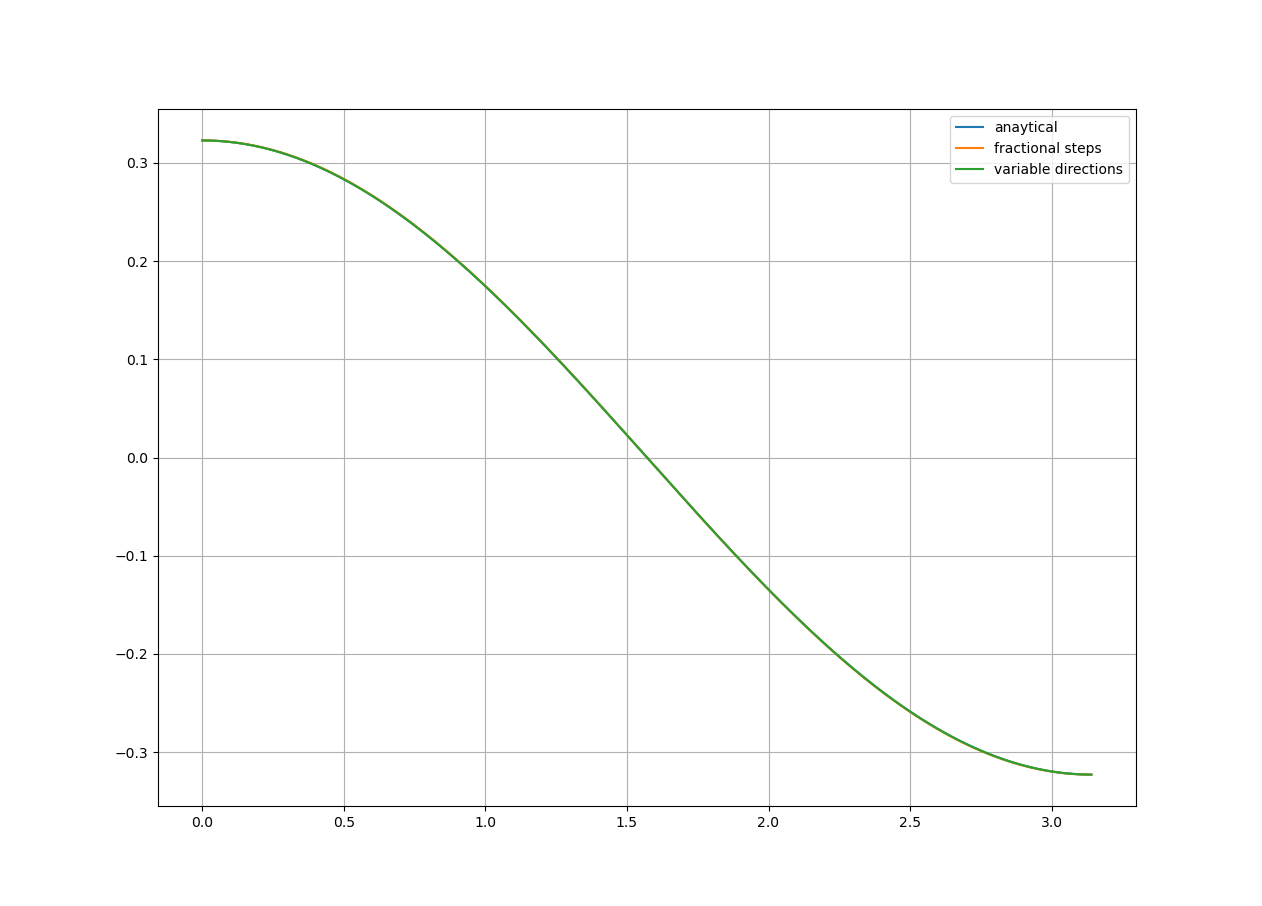
\includegraphics[scale=0.25]{img/img01.png}
\pagebreak
\\
Изменение погрешности
\\
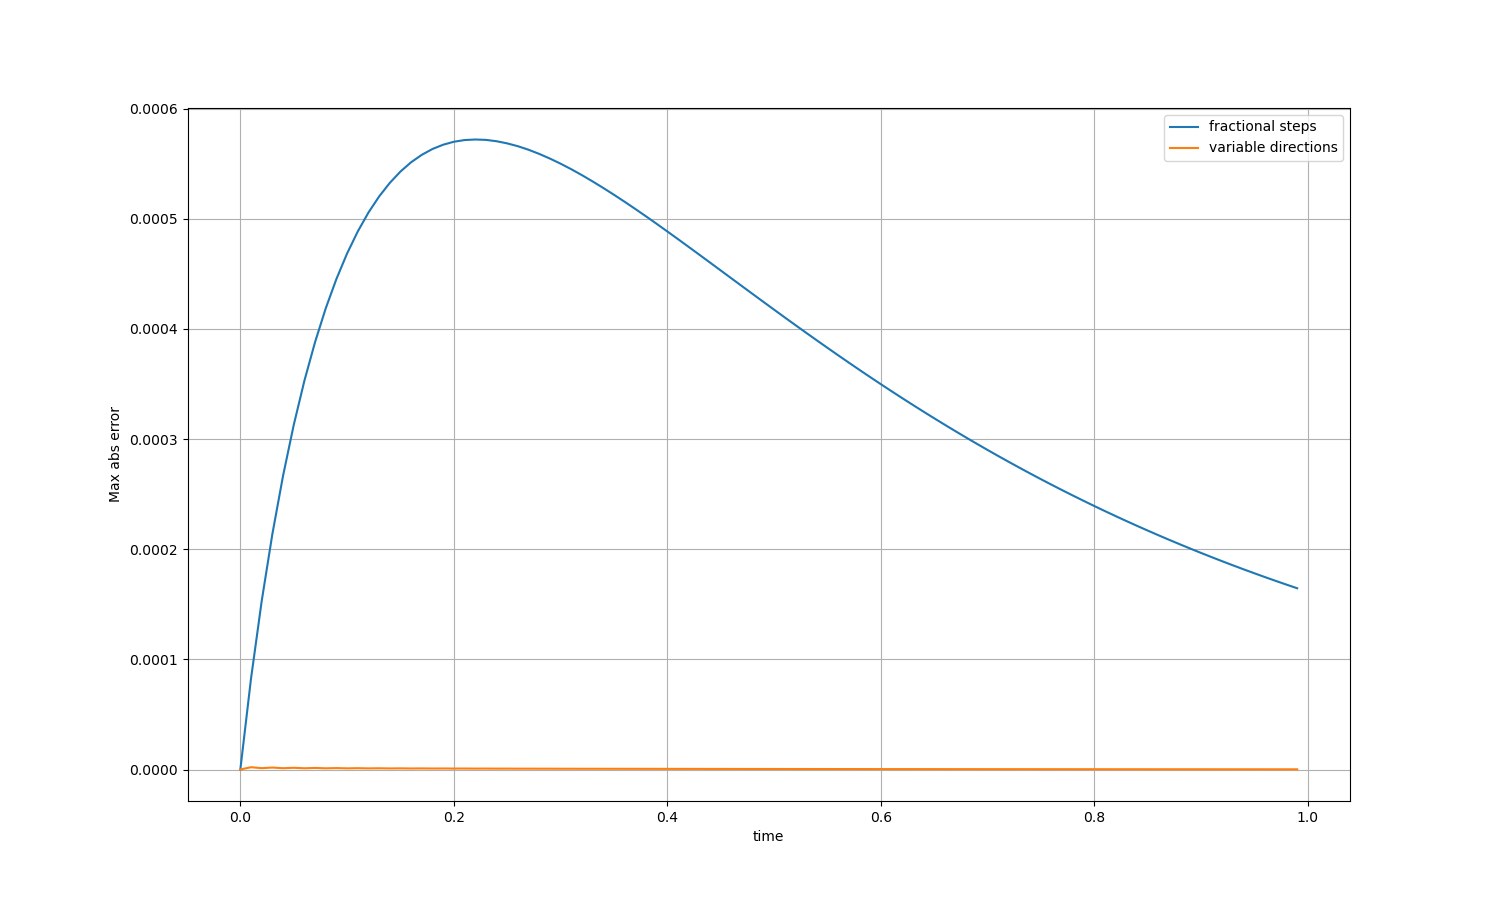
\includegraphics[scale=0.25]{img/img02.png}
\end{center}

\subsection*{Вывод}
Проделав лабораторную работу, я решил начально-краевую задачу для ДУ 
параболического типа и проверил погрешности полученных вычислений.

\end{document}
